\chapter{微流控线虫芯片的设计及硬件平台的搭建}
\section{引言}
	
	在传统的药物筛选过程中,往往是通过人工的方式在96孔板上配置不同浓度的化合物。
	然后将线虫暴露在不同浓度的化合物下,观察并记录线虫在不同浓度化合物下的变化。
	这种人工稀释的方法不仅存在样品消耗大、通量低和操作繁琐等缺点,而且也不利于
	观察。近年来,随着微流控技术的发展,一些研究者们提出了基于微流控技术的片上浓度稀释的方法。
	片上浓度梯度稀释的方法不仅使反应体系减小十倍甚至百倍,
	而且极大的减少了试剂的消耗,节约了实验成本。虽然已经有“圣诞树”结构的被动式梯度
	形成芯片的报道,但存在样品消耗大以及需要精确的流阻设计和流速调节。
	为了研究多种化合物的复合对线虫活性的影响,
	本文设计了一种基于振荡的线性梯度稀释的微流控芯片。且只需要一个气源即可通过振荡的方式
	完整样品的快速稀释,并通过染料实验和荧光实验验证本文提出的线性浓度梯度芯片的可行性。
	
\section{线虫芯片的设计与验证}
\subsection{线虫梯度芯片的设计}
\label{arch-design}
\begin{figure}[htbp]
	  \centering
	  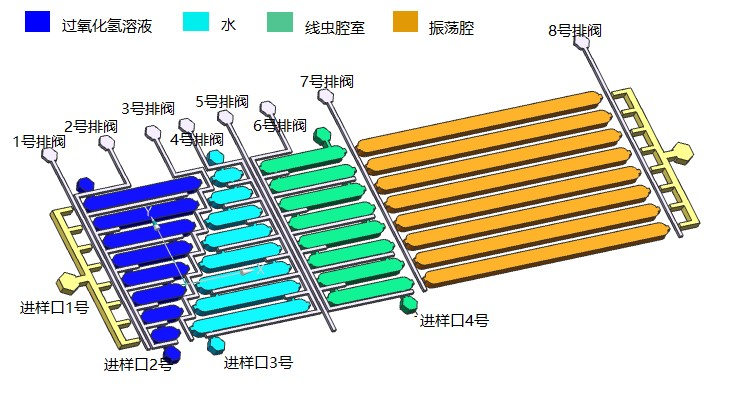
\includegraphics[width=13cm]{figure/chap2/chip-arch.jpg}
	  \bicaption[这里将出现在插图索引中]
		{线性梯度稀释芯片结构}
		{Structure of Linear gradient dilution chip}
	  \label{fig:chap2:chip-arch}
	\end{figure}
线虫梯度芯片的设计如图\ref{fig:chap2:chip-arch}所示,由两层PDMS管道组成。上层为流道层,下层为阀门层。
芯片包含八个阀门和四个进样口。阀门分别控制每列之间的隔绝和开启以及每列腔室之间的相互隔绝和开启。
其中3、5、7号阀门控制4列每列之间的隔绝,而2、4、6号阀门分别控制1、2、3列里9排腔室之间的隔绝,8个阀门将整个芯片分为$9\times4$个独立的腔室。
4列腔室中第一列腔室的长度依次线性递减,第二列腔室的长度依次线性增加,前两列腔室的长度总和为2mm (两腔室长度的比例从上到下依次为$9:1,8:2,\dots,1:9$)。
第三列和第四列腔室的长度保持恒定分别为1mm和3mm。所有腔室的宽度和高度分别为200um和80um。

\subsection{实验材料与仪器}
	\begin{table}[htbp]
	\centering
	\bicaption[指向一个表格的表目录索引]
    {实验试剂与耗材}
    {Experimental reagents and consumables}
	\begin{tabular}{p{150pt}p{230pt}}
	\toprule
		光刻胶SU-83050 & 美国Microchem公司\\
		光刻胶AZ4903 & 德国Merck Performance Materials公司\\
		聚二甲基硅氧烷PDMS( polydimethylsiloxame, RTV 615) &美国 Momentive Performance Materials 公司\\
		氟化液FC-40 & 北京伊诺凯科技有限公司\\
		FA1004分析电子天平 & 上海良平仪器仪表有限公司\\
		RC8型匀胶机 & 美国 Karl Suss公司\\
		DZF-6020型真空干燥箱& 上海新苗医疗器械制造有限公司\\
		ZXZ-2型旋片式真空泵 & 浙江谭氏真空设备有限公司\\
		SMZ-168型体式显微镜& 中国麦克奥迪公司 \\
	\bottomrule
	\end{tabular}
	\end{table}
\subsection{芯片模具加工工艺}
\subsubsection{阀门层模具制作}
	
	\begin{enumerate}[label={\alph*)},font={\color{black!50!black}\bfseries}]
	\item 按照\ref{arch-design}小节的结构设计使用AutoCAD绘图软件绘制阀门层的结构图案并制作掩模版。
	\item 在涂胶之前,需先将3英寸的单抛硅片放在180$^\circ C$的烘箱中2小时,然后用氧等离子体去胶机处理60秒。
	\item 旋涂光刻胶AZ4903并用200rpm的转速预转8秒,然后再用1000rpm的转速甩胶25秒得到22um厚的胶。
	\item 将硅片放入烘箱中,逐渐升温至$50^\circ C$,30分钟后再将温度升高至$90^\circ C$,90分钟后再将其取出。
	\item 经过紫外曝光后再显影。
	\item 为了去除硅片表面的水汽,将其放入$80^\circ C$的烘箱中1小时,最后使用甲基三氯硅烷处理硅片表面5分钟。
	\end{enumerate}
	
\subsubsection{流道层模具制作}
	由于本文中芯片的管道和腔室的高度被设计成不同的尺寸,且腔室的高度要比管道的高度要高,
	所以需要经过两次光刻才能完成流道层模具的制作,第一次光刻采用正胶制作管道结构,第二次光刻采用负胶制作腔室结构。
	\begin{enumerate}[label={\alph*)},font={\color{black!50!black}\bfseries}]
	\item 使用AutoCAD绘图软件分别绘制芯片管道和芯片腔室的结构并打印制作掩模。
	\item 在涂胶之前,需先将3英寸的单抛硅片放在180$^\circ C$的烘箱中2小时,然后用氧等离子体去胶机处理60秒。
	\item 旋涂光刻胶AZ4903并用200rpm的转速预转8秒,然后再用1000rpm的转速旋涂25秒得到22um厚的胶。
	\item 将硅片放入烘箱中,逐渐升温至$50^\circ C$,30分钟后再将温度升高至$90^\circ C$,90分钟后再将其取出。
	\item 经过紫外曝光后再显影。
	\item 将硅片放在热板上分别升高温度分别在$65^\circ C$、$95^\circ C$、$120^\circ C$和$190^\circ C$分别停留
	5min、5min、40min和60min。
	\item 旋涂负胶SU-8 3050并用500rpm的转速预转8秒,然后再用1500rpm的转速旋涂30秒得到80um厚的胶。
	\item 将硅片放在$95^\circ C$的烘箱中恒温40min。
	\item 经紫外曝光后将硅片放入$95^\circ C$的烘箱中恒温60min。
	\item 用对应的显影液对硅片显影,并用异丙酮溶液漂洗,以除去残留的显影液和试剂残留并用氮气将硅片吹干。
	\item 为了除去水汽,将硅片放入$80^\circ C$的烘箱中恒温60min,再用甲基硅氧烷处理5min。
	\end{enumerate}
\subsection{线虫梯度芯片的制作}
	制作好芯片模具后,就可以利用芯片模具进行微流控芯片的制作,下面将介绍双层微流控芯片的制作流程。经过以下流程
	最终完成的芯片其实物图如图\ref{fig:chap2:chip-fabric}所示,为了更好的显示芯片结构,芯片的四列腔室
	都被打入不同颜色的染料。
	\begin{enumerate}[label={\alph*)},font={\color{black!50!black}\bfseries}]
	\item 将流道层硅片的背面用胶粘在一次性培养皿的底部,起到一个固定的作用。
	\item 配制PDMS:按照20:1的比例,取20克RTV 615(A液)和1克固化剂(B液)混合搅拌均与,按照5:1的比例,
	取20克RTV 615(A液)和4克固化剂(B液)混合搅拌均匀,并将两种比例的混合液放入真空皿中抽真空以排出液体中的气泡,
	不断地抽气放气直到液体呈现澄清状。
	\item 将5:1的PDMS混合液倒入流道层培养皿中,PDMS混合液的厚度大约5mm左右。
	\item 将阀门层硅片放在甩胶机吸盘的中心位置,并用真空吸住硅片使其固定,将20:1的PDMS混合液倾倒在硅片上,
	用400rpm的转速预转20秒后再用1800rpm的转速转60秒即可得到厚约40um的PDMS层。
	\item 将阀门层模具和流道层模具一起放入$80^\circ C$的烘箱中恒温30min。
	\item 用手术刀将培养皿中的PDMS层沿着硅片的边沿切下并取出。再用铲刀沿着芯片上的图案将其切成长方形。
	\item 在显微镜下将上一步切下的流道层芯片与阀门层对准并粘合在一起。
	\item 将其放入$75^\circ C$的烘箱中恒温5个小时进行高温键合,然后将其取出放在无尘纸上进行常温冷却。
	\item 再用打孔器将芯片的进样口、出样口和阀门入口位置打孔。
	\item 将芯片和干净的玻璃片一起放入氧等离子体去胶机中处理40秒后,将芯片和玻璃贴合在一起并放入$80^\circ C$的烘箱中
	恒温2小时。
	\end{enumerate}
	\begin{figure}[htbp]
	  \centering
	  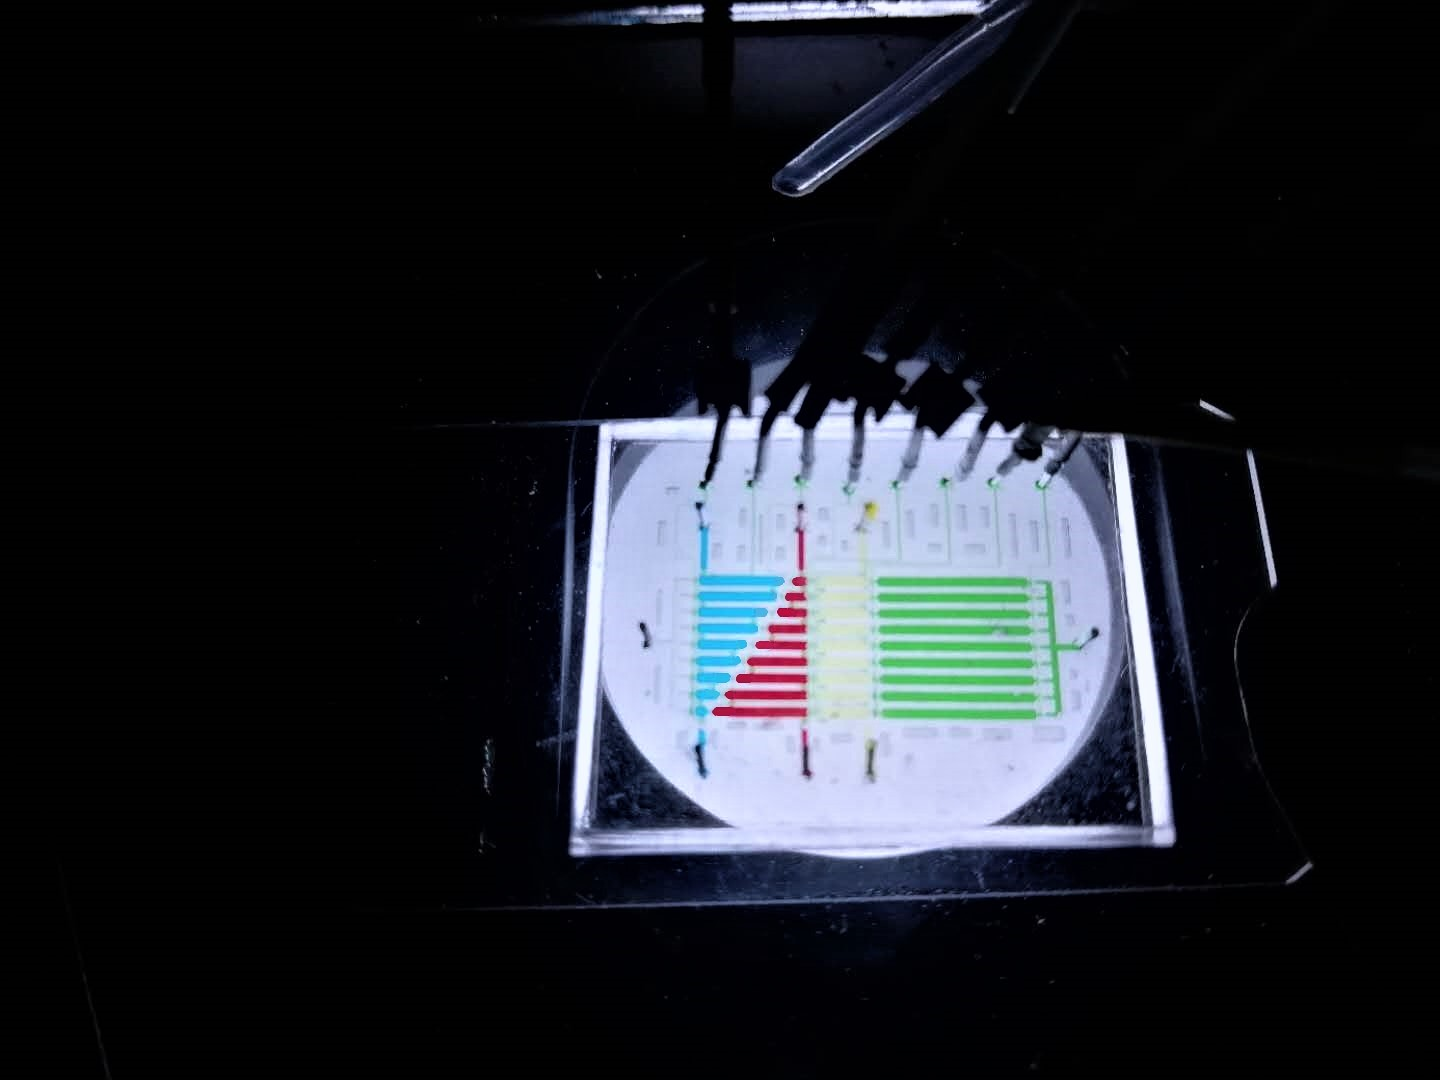
\includegraphics[width=9cm]{figure/chap2/fabric-chip.jpg}
	  \bicaption[这里将出现在插图索引中]
		{线性梯度稀释芯片实物图}
		{fabricated linear gradient dilution chip}
	  \label{fig:chap2:chip-fabric}
	\end{figure}
\section{基于振荡的梯度稀释方法}
\subsection{振荡的理论机制}
	在微流控芯片中,流体的雷诺系数Re变得很小,流体以层流的方法流动,
	这使得微管道中的不同液体的混合变得非常缓慢。我们课题组提出了一种只需一个压力源的基于流体振荡的混合器\cite{cheng2018simple},
	振荡的时候需要在管道的一端构造一个封闭的空腔环境。当需要混合前两列腔室中的液体时,需要将第三列作为储气腔,
	将第三列腔室右边的阀门关闭即可形成封闭的储气腔。当需要混合前三列腔室中的液体时可以将第四列腔室作为储气腔。
	振荡的时候将九排腔室之间的阀门关闭,对其中一排腔室的受力分析可等效为图\ref{fig:force},
	其中$P_{atm}$、$P_{push}$和$P_{air}$分别表示大气压、外部施加的压强与大气压的差和储气腔中的气压。
	储气腔由于封闭了一段空气,当开始施加外部压力时,此时外部气压大于储气腔内的气压,
	会推动液体往储气腔运动,储气腔内的气体由于受到液体的挤压,体积会收缩且内部压强开始增大;
	当外部压力撤掉时,由于储气腔中的压强大于外部的压强,液体会向反方向运动,
	这时储气腔的体积会增大压强会变小。当压强下降到等于外部压强时,液体会停止向前运动,继续施加压力,
	液体又会重复上述运动,这样液体会在周期性气压的作用下来回振荡,类似于宏观的混合吹打从而完成不同溶质的混合。
	\begin{figure}[!htp]    
	\begin{minipage}[t]{0.5\linewidth}%设定图片下字的宽度,在此基础尽量满足图片的长宽    
		\centering    
		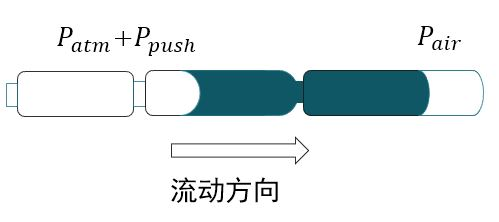
\includegraphics[width=1\linewidth]{figure/chap2/force2.jpg}    
		\caption*{(a) 压缩过程受力分析}%加*可以去掉默认前缀,作为图片单独的说明    
		\label{fig:compress}    
	\end{minipage}    
	\begin{minipage}[t]{0.5\linewidth}%需要几张添加即可,注意设定合适的linewidth    
		\centering    
		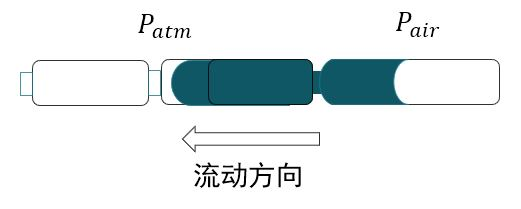
\includegraphics[width=1\linewidth]{figure/chap2/force1.jpg}    
		\caption*{(b) 解压缩过程受力分析}
		\label{fig:decompress}
	\end{minipage}
	\bicaption{液体振荡过程受力分析}{ Stress analysis of liquid oscillation process}%n张图片共享的说明
	\label{fig:force}
	\end{figure}
	
\subsection{染料与荧光实验}
为验证振荡混合效果,我们使用染料及荧光进行验证。如图\ref{fig:before}所示,将第一列腔室打入红色染料,
第二列腔室打入水,将第三列腔室作为振荡腔。在1号进样口施加一个周期为250ms压力值为0.05Mpa的气压,
经过7分钟的振荡,染料已经充分的混合均匀。染料和水完全混合后的效果如图\ref{fig:after}所示,从上到下染料的颜色依次变淡。
如不加振荡,两列液体以自由扩散方式混合,需要2~3个小时,可以看出,振荡方法对快速混合形成梯度有较好的效果,
大大加快了不同液体的混合速率。
为了定量的验证梯度形成的准确性,我们将第一列腔室中的染料替代为浓度为0.1g/L 的荧光素钠溶液(pH=7),
最终得到0.01~0.09g/L的线性浓度梯度。图\ref{fig:chap2:fluence}为荧光素钠浓度与荧光强度之间的关系。
图中蓝色的线表示线性拟合的结果,可以看出拟合结果的线性度较好。
从而验证了基于微振荡原理的大规模梯度稀释是可行的,
这种方式能够显著加快混合的速度并且只需要一个压力源即可完成振荡混合。
为了验证这种振荡对线虫并无不良后果,我们将线虫打入第三列腔室,并在该参数下振荡,
观察2个小时发现线虫的摆动频率并没有出现太大波动。

	\begin{figure}[!htp]
	\centering
	  \begin{subfigure}{0.45\textwidth}
		\centering
		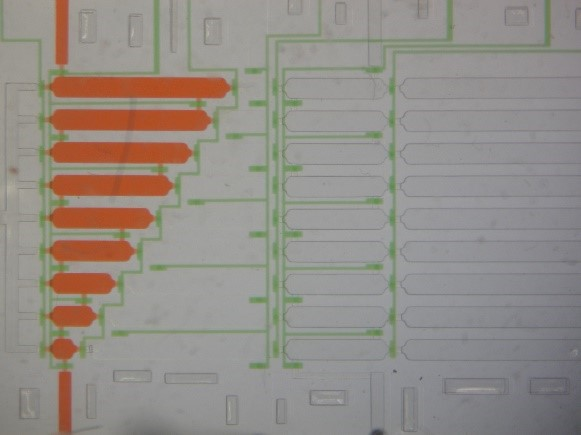
\includegraphics[width=1\linewidth]{figure/chap2/before.jpg}
		\caption{振荡前的芯片图 }
		\label{fig:before}   
	  \end{subfigure}
		\hspace{1em}
	  \begin{subfigure}{0.45\textwidth}
		\centering
		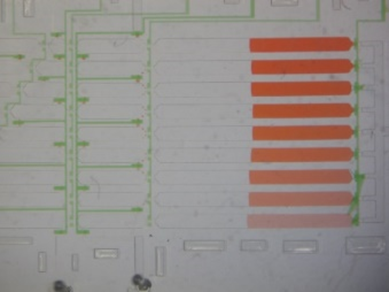
\includegraphics[width=1\linewidth]{figure/chap2/after.png}
		\caption{振荡结束后的芯片图}
		\label{fig:after}
	  \end{subfigure}
	  \bicaption{染料实验结果}{Dye experiment results}
	  \label{fig:oscillation}
	\end{figure}

	\begin{figure}[htbp]
	  \centering
	  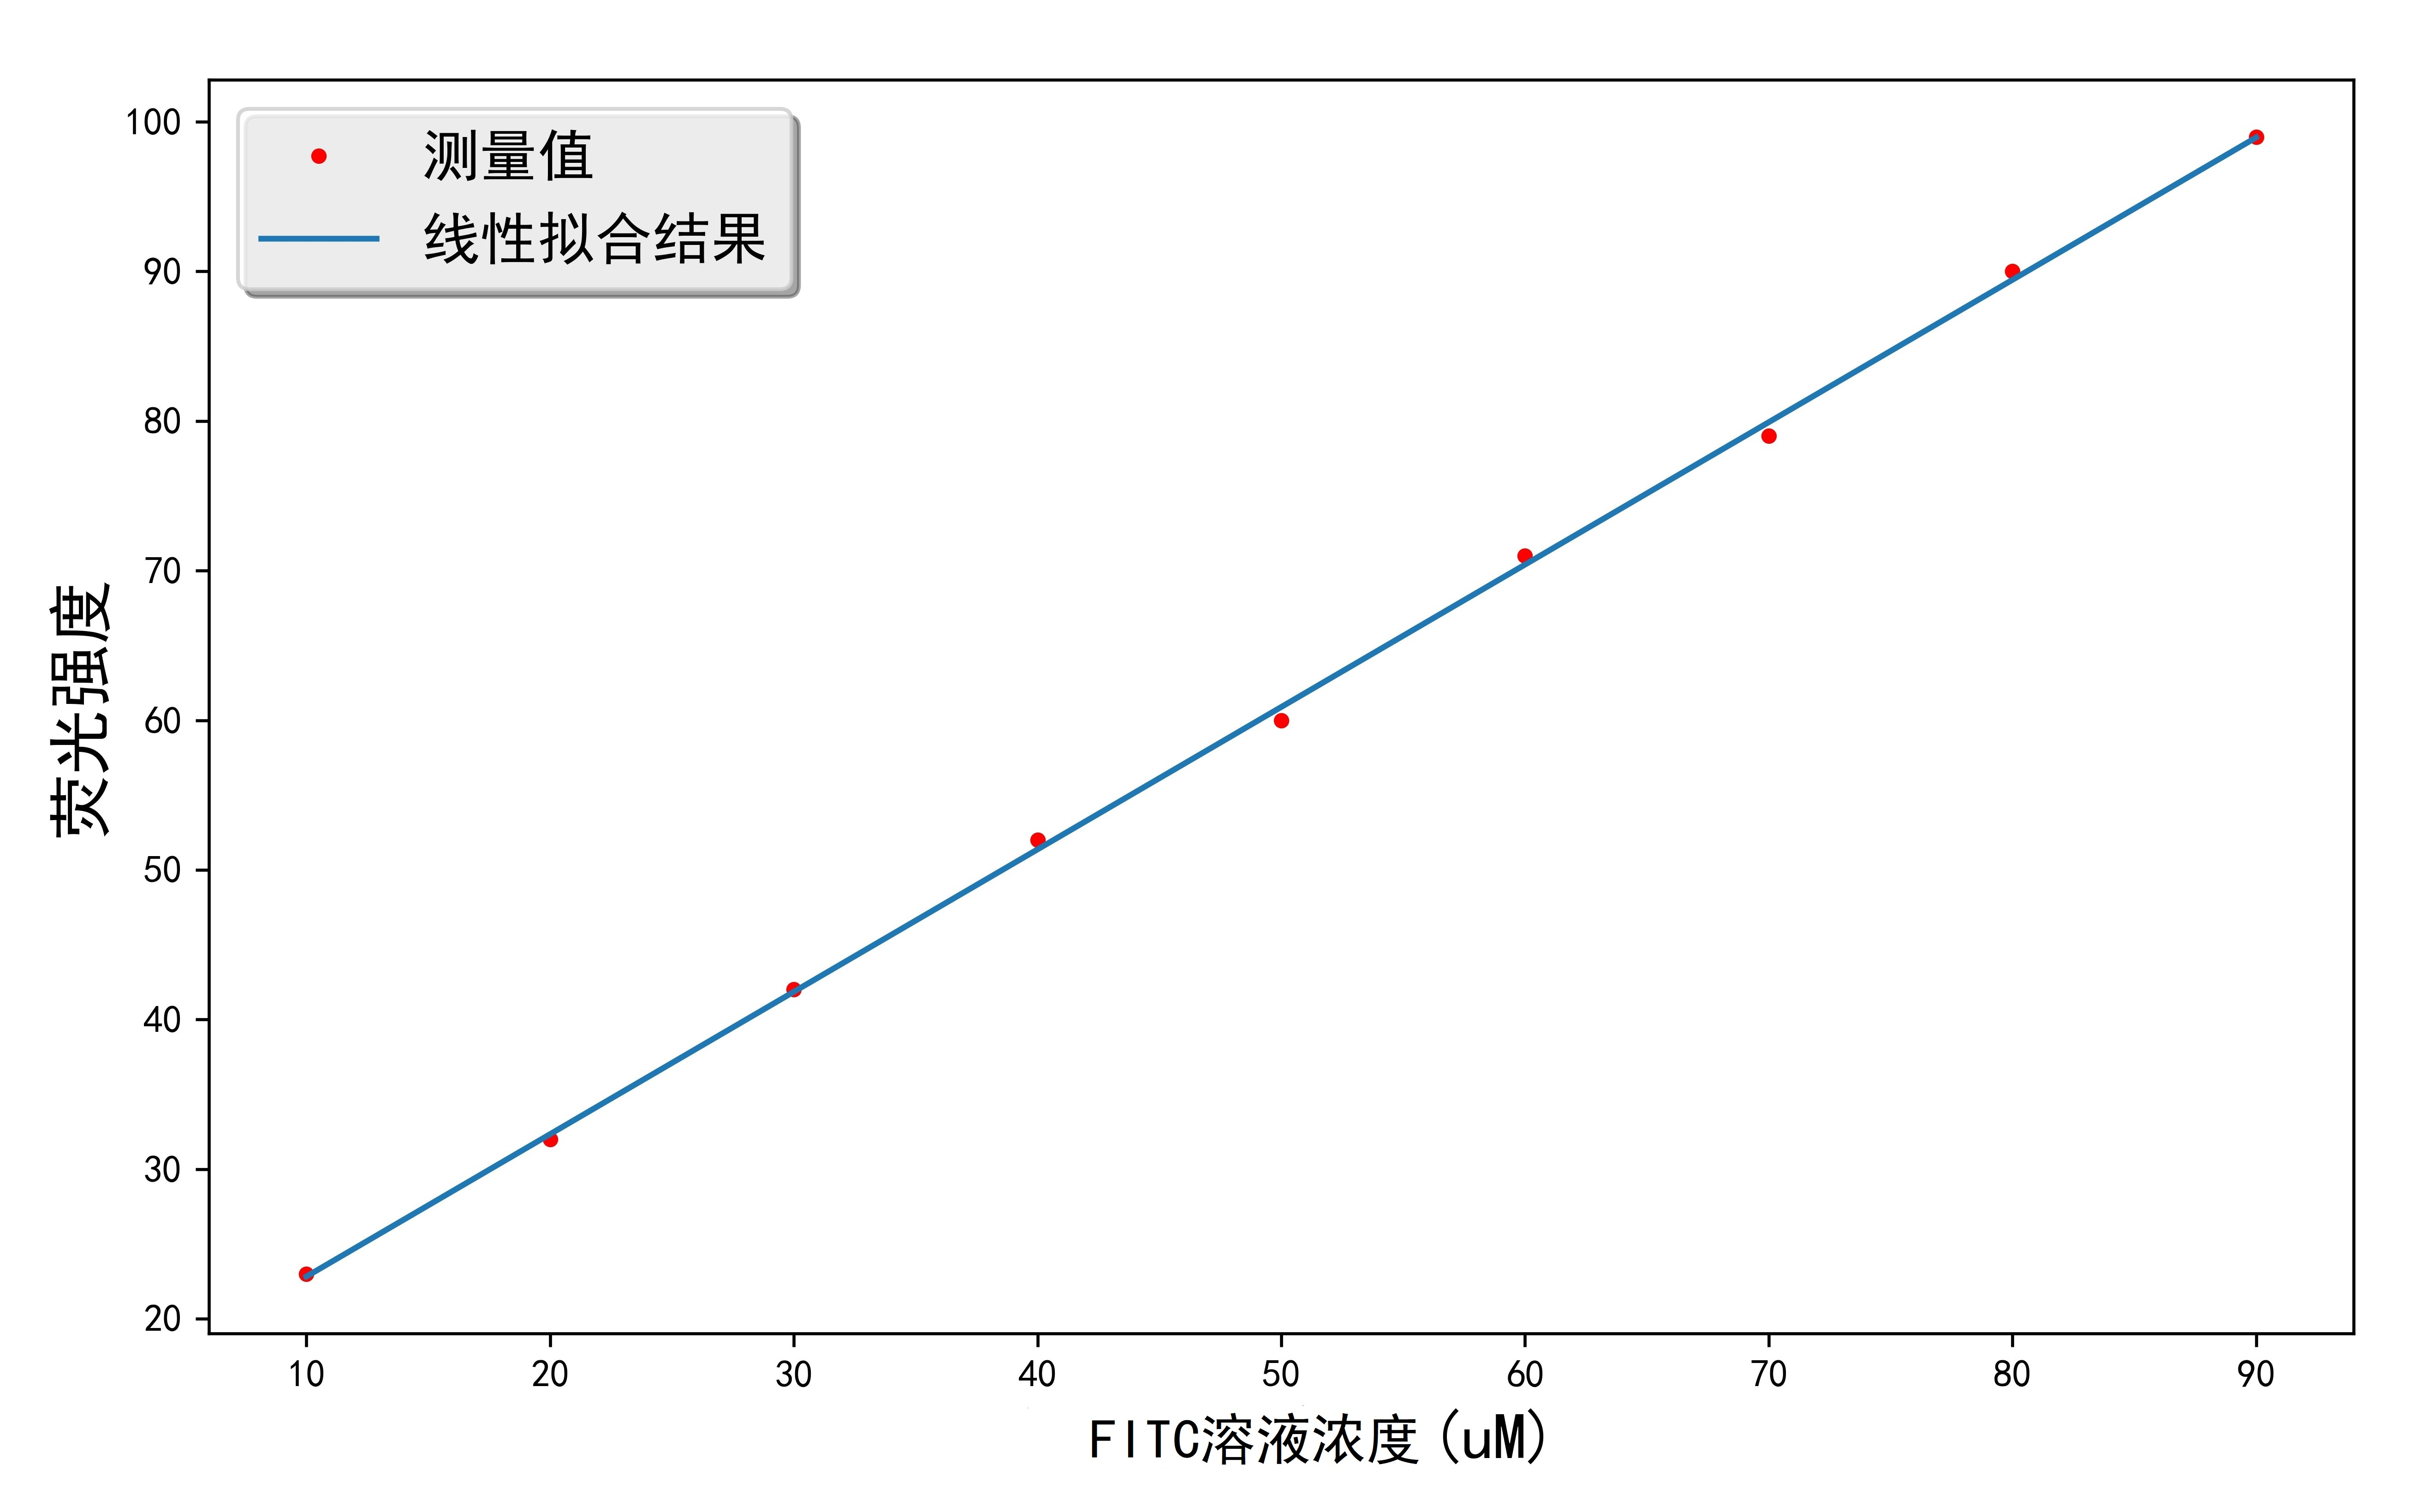
\includegraphics[width=9cm]{figure/chap2/fluence.jpg}
	  \bicaption[这里将出现在插图索引中]
		{荧光实验结果}
		{Fluorescence experiment results}
	  \label{fig:chap2:fluence}
	\end{figure}
\section{阀门控制系统搭建}
	目前,双层的微流控芯片一般由下层的阀门层和上层的流道层组成。阀门层的PDMS薄膜通常很薄,当向气阀通道施加一定的
	气压(大约30psig),阀门层的薄膜会向上顶起。由于上层的流道和下层的气阀通道是上下交叉的,通过控制向气阀通道施加
	气压,便可以控制上层流道的通断。另一方面,线虫的压力进样和芯片的振荡都需要对进样口进行气压控制。基于以上需求
	,本课题组开发了自动化阀门控制系统,图\ref{fig:flow_chart}为该系统的连接示意图。整个系统由五个模块构成,
	我们采用了750W-18L小型空压机作为气泵模块为整个系统提供气压输出,将Arduino作为微控制器控制电磁阀的输出。
	Arduino由运行在电脑上的上位机程序控制。

	\begin{figure}[!htp]
    \centering
	
    \begin{tikzpicture}[node distance=2.5cm,auto]
	\tikzstyle{process} = [rectangle,rounded corners,thick,minimum width = 3cm,text width=3cm,inner sep=2pt,minimum height =1.7cm, text centered, draw = black]
    \node (pc) [process] {电脑};
    \node (mcu) [process, below of=pc] {微控制器及运算放大器};
    \node (valves) [process, below of=mcu] {电磁阀};
    \node (pump) [process, right of=valves,node distance=4cm] {气泵};
    \node (chip) [process, left of=valves,node distance=4cm] {微流控芯片};
    %连接具体形状
    \draw [arrow](pc) -- (mcu);
    \draw [arrow](mcu) -- (valves);
    \draw [arrow](valves) -- (chip);
    \draw [arrow](pump) -- (valves);
	\end{tikzpicture}
    \bicaption{自动化阀门控制系统}{Automated valve control system}
    \label{fig:flow_chart}
	\end{figure}
\section{高速视频采集程序的设计}
	线虫视频的高速采集对线虫摆动频率的估计是至关重要的一步。根据采样定理,采集的视频帧率至少是线虫摆动频率的两倍。
	除了采样频率的要求外,视频的分辨率等因素同样影响后续线虫图像处理的难度。基于以上考虑,本文选取鑫图公司的DigiRetina 16
	 COMS相机作为线虫视频的采集模块。其可以通过USB3.0高速传输接口与电脑进行高速图像数据传输,同时该相机在放大倍率20
	 倍以下的显微成像中,也可以获得分辨率优异的显微图像,另外其内置两个FPGA双核处理器分别用于高清图像处理和
	 图像输出控制。该相机较好满足了本文对线虫视频采集模块的要求。为了提高视频采集的帧率,本文基于该相机的SDK,开发基于多线程
	 的视频采集程序。
	 
	对DigiRetina 16相机设备的操作通常分为7个步骤,其操作流程如图\ref{fig:flow_chart1}所示。设备初始化阶段主要负责和相机驱动通信并对其
	初始化,在图像采集之前,需要在内存中开辟内存空间用于保存采集的图像数据,所需内存的大小与图像的分辨率有关。
	DigiRetina 16相机支持多种分辨率的图像采集,分辨率可以在打开设备后进行设置。在结束采集后,需要关闭设备并
	释放内存空间。
	\begin{figure}[!htp]
    \centering
    \begin{tikzpicture}[node distance=2.5cm,auto]
	\tikzstyle{process} = [rectangle,rounded corners,thick,minimum width = 3cm,text width=3cm,inner sep=2pt,minimum height =1.5cm, text centered, draw = black]
    \node (init) [process] {设备初始化};
    \node (allocate) [process, right of=init,node distance=4cm] {分配内存空间};
    \node (open) [process, right of=allocate,node distance=4cm] {打开设备};
    \node (op) [process, below of=open,yshift=0.5cm] {图像采集};
    \node (close) [process, below of=op,yshift=0.5cm] {关闭设备};
	\node (free) [process, left of=close,node distance=4cm] {释放内存空间};
	\node (exit) [process, left of=free,node distance=4cm] {释放驱动};
    %连接具体形状
    \draw [arrow](init) -- (allocate);
    \draw [arrow](allocate) -- (open);
    \draw [arrow](open) -- (op);
    \draw [arrow](op) -- (close);
	\draw [arrow](close) -- (free);
	\draw [arrow](free) -- (exit);
	\end{tikzpicture}
    \bicaption{相机设备的操作流程}
	{Camera device operation flow}
    \label{fig:flow_chart1}
	\end{figure}
	\begin{figure}[!htp]
    \centering
    \begin{tikzpicture}[node distance=2.5cm,auto]
	\tikzstyle{rect1} = [rectangle,rounded corners,thick,minimum width = 3cm,fill=green!30,
	text width=3cm,inner sep=2pt,minimum height =2cm, text centered, draw = black]
    \tikzstyle{rect2} = [rectangle,rounded corners,thick,minimum width = 3cm,fill=orange!30,
	text width=3cm,inner sep=2pt,minimum height =2cm, text centered, draw = black]
	\tikzstyle{label} = [rectangle,rounded corners,minimum width = 7cm,text width=7cm,inner sep=2pt,minimum height =1.5cm, text centered, draw = black]
	\tikzstyle{arrow1} = [->, >=latex', shorten >=1pt, thick]
	\tikzstyle{arrow2} = [->, >=latex', shorten >=1pt]
	\node (node1) [rect1] {等待一帧图像,时间开销T1};
    \node (node2) [rect1, right of=node1,node distance=4cm] {从相机设备内存到电脑内存的复制,时间开销T2};
    \node (node3) [rect2, right of=node2,node distance=4cm] {图像处理程序从电脑内存中读取图像,时间开销T3};
    \node (node4) [rect2, right of=node3,node distance=4cm] {处理一帧图像,时间开销T4};
    %连接具体形状
    \draw [arrow1](node1) -- (node2);
    \draw [arrow1](node2) -- (node3);
    \draw [arrow1](node3) -- (node4);
    % \draw [arrow2](node1) -- (label1);
	% \draw [arrow2](node2) -- (label2);
	% \draw [arrow2](node3) -- (label3);
	% \draw [arrow2](node4) -- (label4);
	\end{tikzpicture}
    \bicaption{相机设备的操作流程}
	{Automated valve control system}
    \label{fig:image_process_flow}
	\end{figure}
	
	一帧图像从采集到被处理共分为4步骤,如图\ref{fig:image_process_flow}所示,各部分的时间开销
	分别用$T_1,T_2,T_3,T_4$表示,下面分别对各部分时间开销进行详细分析:
	\begin{description}
    \item[时间开销T1:] 曝光时间和图像分辨率影响这部分的时间开销,增加曝光时间或提高图像采集的分辨率
	都会使这部分的时间开销变大。
    \item[时间开销T2:] 相机驱动程序负责将相机缓存中的图像数据传送到电脑上的一块内存区域。
	这个内存块在相机初始化时开辟,释放相机设备时自动释放,图像采集的分辨率、USB线的长度会影响时间开销。
    \item[时间开销T3:] 图像处理程序从上一步的内存区域读取图像数据。
					图像分辨率、内存拷贝数据的速度等会影响时间开销
	\item[时间开销T4:] 处理一帧图像的时间对不同的图像处理程序而言是不同,这部分的时间开销与具体的图像处理算法
	有关。对于高速视频采集任务而言,这里的时间开销指的是写入硬盘时间。
	\end{description}
	
	\begin{figure}[!htp]
    \centering
    \begin{tikzpicture}[node distance=2.5cm,auto]
	\tikzstyle{rect1} = [rectangle,rounded corners,thick,minimum width = 3cm,fill=green!30,
	text width=3cm,inner sep=2pt,minimum height =2cm, text centered, draw = black]
    \tikzstyle{rect2} = [rectangle,rounded corners,thick,minimum width = 3cm,fill=orange!30,
	text width=3cm,inner sep=2pt,minimum height =2cm, text centered, draw = black]
	\tikzstyle{label} = [rectangle,rounded corners,minimum width = 7cm,text width=7cm,inner sep=2pt,minimum height =1.5cm, text centered, draw = black]
	\tikzstyle{arrow1} = [->, >=latex', shorten >=1pt, thick]
	\tikzstyle{arrow2} = [->, >=latex', shorten >=1pt]
	\node (node1) [rect1] {等待一帧图像,时间开销T1};
    \node (node2) [rect1, right of=node1,node distance=4cm] {从相机设备内存到电脑内存的复制,时间开销T2};
    \node (node3) [rect2, right of=node2,node distance=4cm] {图像处理程序从电脑内存中读取图像,时间开销T3};
    \node (node4) [rect2, right of=node3,node distance=4cm] {处理一帧图像,时间开销T4};
    %连接具体形状
    \draw [arrow1](node1) -- (node2);
    \draw [arrow1](node2) -- (node3);
    \draw [arrow1](node3) -- (node4);
    % \draw [arrow2](node1) -- (label1);
	% \draw [arrow2](node2) -- (label2);
	% \draw [arrow2](node3) -- (label3);
	% \draw [arrow2](node4) -- (label4);
	\end{tikzpicture}
    \bicaption{相机设备的操作流程}
	{Automated valve control system}
    \label{fig:image_process_flow}
	\end{figure}
	
	
	
\section{本章小结}
	本章的主要工作是为本文提出的药物筛选平台搭建了一个硬件平台。首先,介绍了基于振荡原理的线性梯度稀释芯片的结构设计。
	本章还介绍了微流控芯片的制作工艺。然后介绍了振荡混合的理论机制,并在最后通过染料实验和荧光实验证明了线性
	梯度稀释芯片设计的合理性,实验结果显示基于振荡的混合方式能够有效的缩短不同液体的混合时间。